\documentclass[12pt,border=0pt]{standalone}
% tikz/tikz-preamble.tex
% Contains only Tikz-related packages and styles/macros
% input into main.tex

\usepackage{tikz}
\usetikzlibrary{arrows.meta,calc,decorations.markings}

% Grid for alignment, needs \W and \H
\newcommand{\LayoutGrid}{
  \begin{scope}[overlay]
    % thin lines
    \draw[step=0.5cm, line width=0.05mm, black!20]
      (0,0) grid (\W,\H);
    % thick lines
    \draw[step=1cm, line width=0.15mm, black!35]
      (0,0) grid (\W,\H);
    \pgfmathtruncatemacro{\GridW}{floor(\W)}
    \pgfmathtruncatemacro{\GridH}{floor(\H)}
    \foreach \x in {1,...,\GridW}{
      \node[anchor=south east,
            inner sep=0.5pt,
            font=\tiny,
            text=black!50]
        at (\x-0.05,0.05) {\x};
    }
    \foreach \y in {1,...,\GridH}{
      \node[anchor=north west,
            inner sep=0.5pt,
            font=\tiny,
            text=black!50]
        at (0.05,\y-0.05) {\y};
    }
  \end{scope}%
}
\newcommand{\pointsize}{0.08}
% Styles
\tikzset{
  closedboundary/.style={line width=1.2pt},
  openboundary/.style={
    line width=1.2pt,
    dash pattern=on 4pt off 4pt,
    line cap=round
  },
  closedpoint/.style={closedboundary, fill=black, draw=black},
  openpoint/.style={closedboundary, fill=white, draw=black}
}
% Axes around origin
% updated to take 4 arguments 
% X1 to X2, Y3 to Y4
\newcommand{\drawAxes}[4]{%
  \draw[-Stealth] (#1,0) -- (#2,0);
  \draw[-Stealth] (0,#3) -- (0,#4);
}

% arrows
\tikzset{
  patharrow/.style n args={1}{
    thick,
    postaction={
      decorate,
      decoration={
        markings,
        mark=at position #1 with {
          \arrow{Triangle[length=3.5mm, width=2.5mm]}
        }
      }
    }
  },
  patharrow/.default=0.68,
  tangentarrow/.style={
    thick,
    -{Triangle[length=3.5mm,width=2.5mm]}
  }
}


\begin{document}

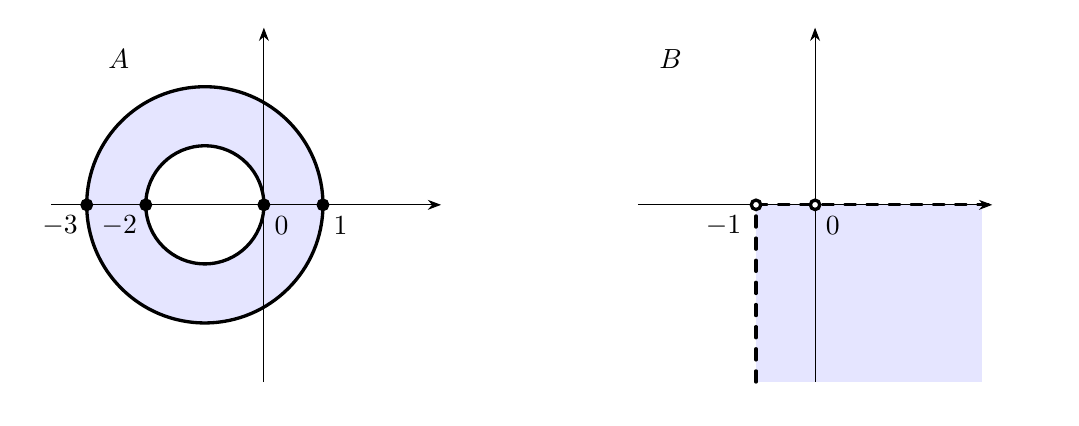
\begin{tikzpicture}[x=1cm,y=1cm]

  \def\W{13}
  \def\H{4.7}
  \path[use as bounding box] (0,0) rectangle (\W,\H);
  % \LayoutGrid

  % A<<<
  \begin{scope}[
    shift={(3,2.45)},
    scale={0.75} % doesn't scale node text
  ]

    \node[anchor=north west] at (-2.8,2.8) {$A$};

    \fill[blue!10] (-1,0) circle (2);
    \fill[white] (-1,0) circle (1);

    \drawAxes{-3.6}{3}{-3}{3}

    \draw[closedboundary] (-1,0) circle (2);
    \draw[closedboundary] (-1,0) circle (1);

    \filldraw[closedpoint] (-3,0) circle (\pointsize);
    \node at (-3.45,-0.35) {$-3$};

    \filldraw[closedpoint] (-2,0) circle (\pointsize);
    \node at (-2.45,-0.35) {$-2$};

    \filldraw[closedpoint] (0,0) circle (\pointsize);
    \node at (0.3,-0.35) {$0$};

    \filldraw[closedpoint] (1,0) circle (\pointsize);
    \node at (1.3,-0.35) {$1$};

  \end{scope}% >>>

  % B<<<
  \begin{scope}[
    shift={(10,2.45)},
    scale={0.75}
  ]

    \node[anchor=north west] at (-2.8,2.8) {$B$};

    \fill[blue!10] (-1,-3) rectangle (2.83,0);

    \drawAxes{-3}{3}{-3}{3}

    \draw[openboundary] (-1,-3) -- (-1,0);
    \draw[openboundary] (-1,0) -- (3,0);

    \filldraw[openpoint] (-1,0) circle (\pointsize);
    \node at (-1.55,-0.35) {$-1$};

    \filldraw[openpoint] (0,0) circle (\pointsize);
    \node at (0.3,-0.35) {$0$};

  \end{scope}% >>>

\end{tikzpicture}

\end{document}
% vim: foldmethod=marker:fmr=<<<,>>>
